\documentclass{beamer}
\usepackage{beamerthemesplit}
\usepackage{hyperref}
\usepackage{color}
\usepackage{listings}
\begin{document}
\title{Hadoop - Distributed Computing for the Masses}
\author{Casey Stella}
\date{\today}

\frame{\titlepage} 

\frame{\frametitle{Table of Contents}\tableofcontents} 

\section{Introduction}

\frame{\frametitle{Hi, I'm Casey}
\begin{itemize}
\item Education
   \begin{itemize}
   \item B.S. in Computer Science from University of Louisiana at Monroe
   \item M.S. in Mathematics from Texas A\&M University with an emphasis in Theoretical Computer Science
   \end{itemize}\pause
\item I tend to work with ``Big Data''
   \begin{itemize}
   \item I just joined Hortonworks as a Systems Architect
   \item I just left the high performance indexing team at Explorys, a medical informatics startup based in the Cleveland Clinic
   \item I was a Research Geophysicist in the Oil Industry doing signal processing
   \item I built a VOIP network oriented toward WoW gamers
   \end{itemize}
\end{itemize}
}

\section{Distributed Computing}

\frame{\frametitle{Distributed Computing}
\begin{itemize}
\item Distributed computing turns out to be hard\pause
   \begin{itemize}
   \item Needs to be fast\pause
   \item Needs to be scalable\pause
   \item Needs to be fault-tolerant\pause
   \end{itemize}
\item Message Passing Systems
   \begin{itemize}
   \item Idea: build your own systems from a set of communication primitives
   \item Often designed specifically to solve one very big, very nasty problem\pause
   \item Pro: very flexible and high performance\pause
   \item Con: can be very difficult to maintain, write and understand.  Designed for massive parallel computers.
   \end{itemize}
\end{itemize}
}

\frame{\frametitle{Map-Reduce}
\begin{itemize}
\item A programming model for processing large data sets in batch.\pause
\item Designed to execute on a cluster of commodity hardware.\pause
\item Let tasks fail and be able to retry.\pause
\item Bring the code to the data, rather than the data to the code.\pause
\item Limit communication to only a certain set of operations.\pause
\item Inspired by functional programming
\end{itemize}
}

\frame{\frametitle{Data Flow}
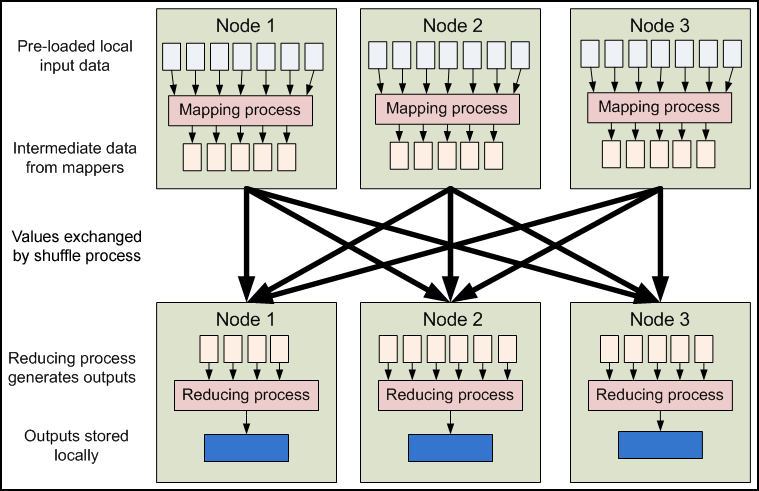
\includegraphics[scale=0.32]{map-reduce.png}\footnote[1]{\url{http://developer.yahoo.com/hadoop/tutorial/module4.html} }
}

\frame{\frametitle{Word Count - The Canonical Example}
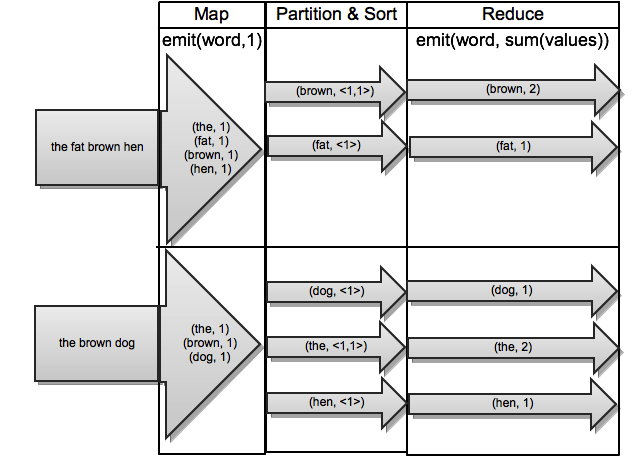
\includegraphics[scale=0.45]{map-reduce-wordcount.png}
}

\frame{\frametitle{Caveats}
\begin{itemize}
\item All problems do not fit well (or at all) within this model.\pause
\item This model is not suitable for real-time processing of data.\pause
\item While it can linearly scale out in relation to your input data, if you choose the number of keys you emit from your mappers improperly, you could create a non-linear scale-out.\pause
\item Easier than rolling your own solution, but can be tricky to fit your problem to it.
\end{itemize}
}

\section{Apache Hadoop}

\frame{\frametitle{History}
\begin{itemize}
\item Hadoop was derived from Google's MapReduce and Google File System (GFS) papers.\pause
\item Open source, Apache licensed project created by Doug Cutting and Michael J. Cafarella.\pause
\item Named after Doug's son's toy elephant.\pause
\item It was originally developed to support distribution for the Nutch search engine project.\pause
\item Has grown to have a whole ecosystem around it: HBase, HDFS, etc.
\end{itemize}
}


\frame{\frametitle{The Components}
\begin{itemize}
\item Zookeeper - Configuration, synchronization and naming registry for distributed systems
\item HDFS - An append-only distributed filesystem inspired by Google File System
\item Hadoop Map-Reduce - The Map-Reduce infrastructure
\item HBase - A column-store NoSQL database inspired by Google BigTable
\end{itemize}
}

\frame{\frametitle{Usage}
\begin{itemize}
\item Core part of Netflix's analytics stack
\item Facebook is a heavy user of map-reduce and HBase runs Facebook's messaging platform
\item Yahoo! continues to be a heavy user
\item O'Reilly Strata and Hadoop World merged this year.  Over 2500 attendees.
\end{itemize}
}

\section{Conclusion}

\frame{\frametitle{Conclusion}
\begin{itemize}
\item Thanks for your attention
\item Follow me on twitter $@casey\_stella$
\item Find me at
  \begin{itemize}
  \item \url{http://caseystella.com}
  \item \url{https://github.com/cestella}
  \end{itemize}
\end{itemize}
}

\end{document}
